\input{mmd-beamer-header-11pt}
\def\mytitle{Reduced Order Modelling for Solar System Barycentring}
\def\mydate{12 July 2017}
\def\myauthor{Matthew Pitkin}
\def\affiliation{University of Glasgow}
\def\latexxslt{beamer}
\def\latexmode{beamer}
\def\theme{m}
\def\event{LIGO-G1701327}
\input{mmd-beamer-begin-doc}


% A presentation to the LVC CW group on using reduced order modelling to speed up solar
% system barycentring time delay calculations
%
% Note: comments can be included in the LaTeX file by surrounding them with html style comment
% blocks and a % sign


\begin{frame}

\frametitle{Background}
\label{background}

The phase evolution of a continuous gravitational wave signal arriving at a detector on
Earth can be written in the form:
\[
\phi(t) = \phi_0 + 2\pi \left(f_0\left[t+\tau(t)\right] + \frac{\dot{f}}{2}\left[t + \tau(t)\right]^2 \ldots \right),
\]
where $t$ is the time at the detector, and $\tau(t)$ is the time delay between the signal arrival
at the detector and the signal arrival at the solar system barycentre (SSB)\footnote{in, e.g., the  \href{https://en.wikipedia.org/wiki/Barycentric_Dynamical_Time}{TDB} coordinate time standard}.

\end{frame}

\begin{frame}

\frametitle{Background}
\label{background}

The time delay term depends on the location of the source, and the position and velocity of the detector with
respect to the SSB, and comprises:
\[
\tau(t) = \Delta T_{\rm R}(t) + \Delta T_{\rm E} - \Delta T_{\rm S}, 
\]
where:

\begin{itemize}
\item $\Delta T_{\rm R}(t)$ is the geometric Roemer delay

\item $\Delta T_{\rm E}$ is the relativistic Einstein delay

\item $\Delta T_{\rm S}$ is the Shapiro delay

\end{itemize}

\end{frame}

\begin{frame}

\frametitle{Background}
\label{background}

Shapiro delay and Einstein delay over one year for source at: $\alpha=0^{\rm h}0^{\rm m}0.0^{\rm s}$, $\delta = 0^{\circ}0'0''.0$

\begin{figure}[htbp]
\centering
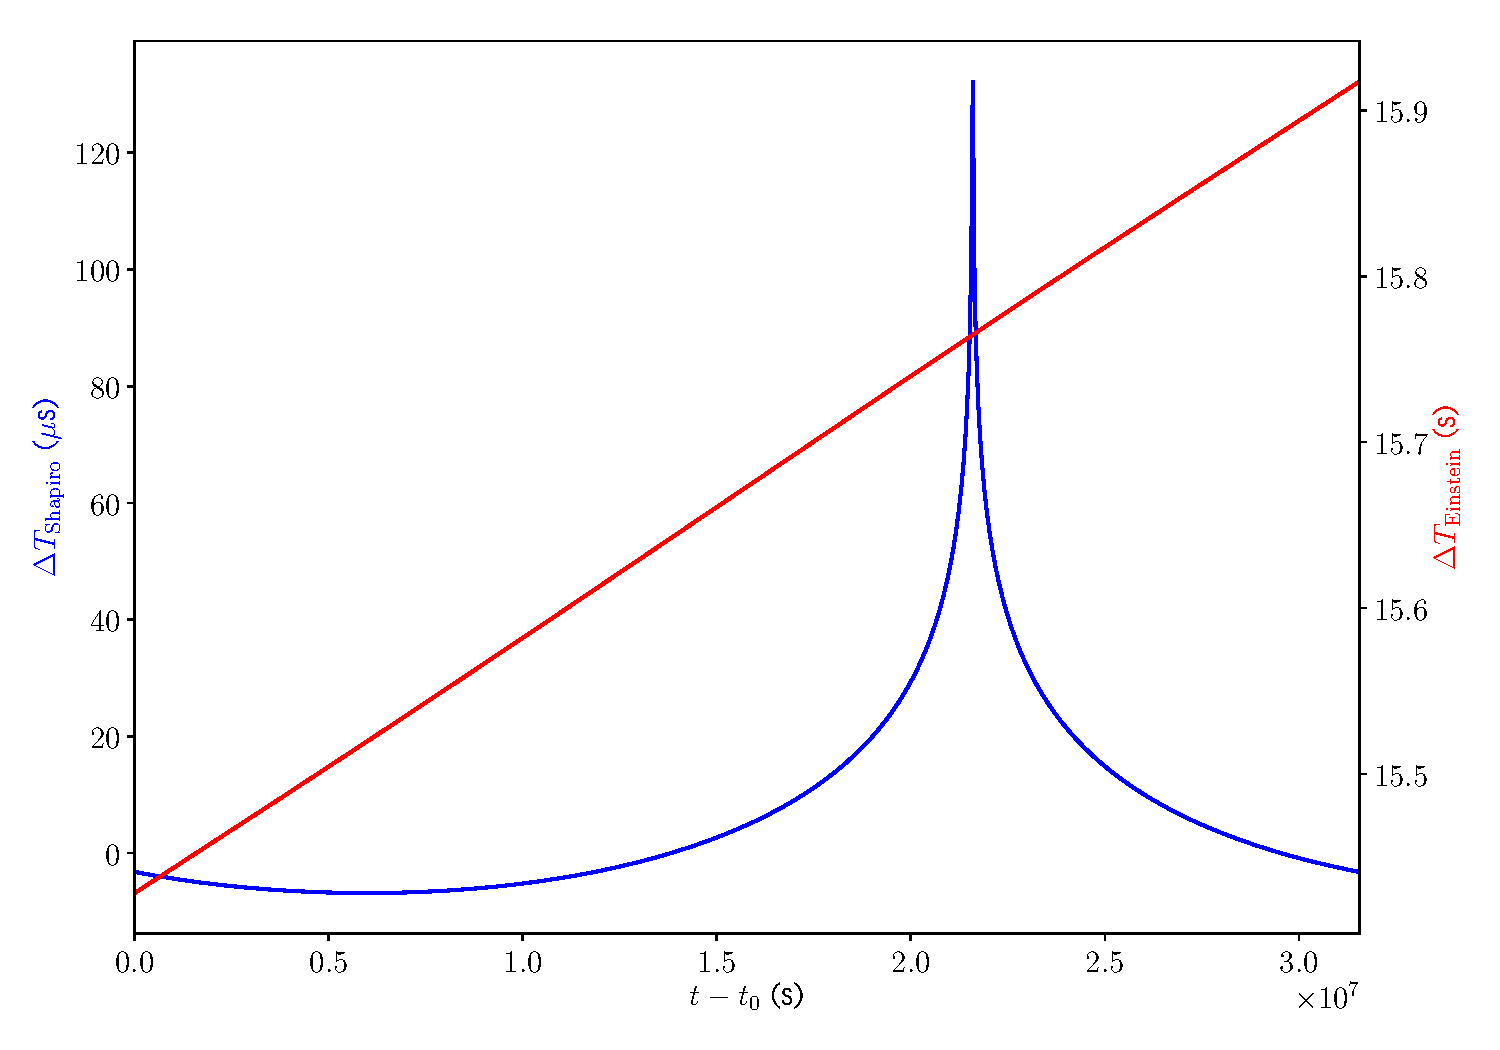
\includegraphics[keepaspectratio,width=\textwidth,height=170pt]{images/shap_ein_delay.pdf}
\label{shap_ein}
\end{figure}

\end{frame}

\begin{frame}

\frametitle{Background}
\label{background}

Roemer delay (over one month) between Earth and SSB, and H1 and geocentre

\begin{figure}[htbp]
\centering
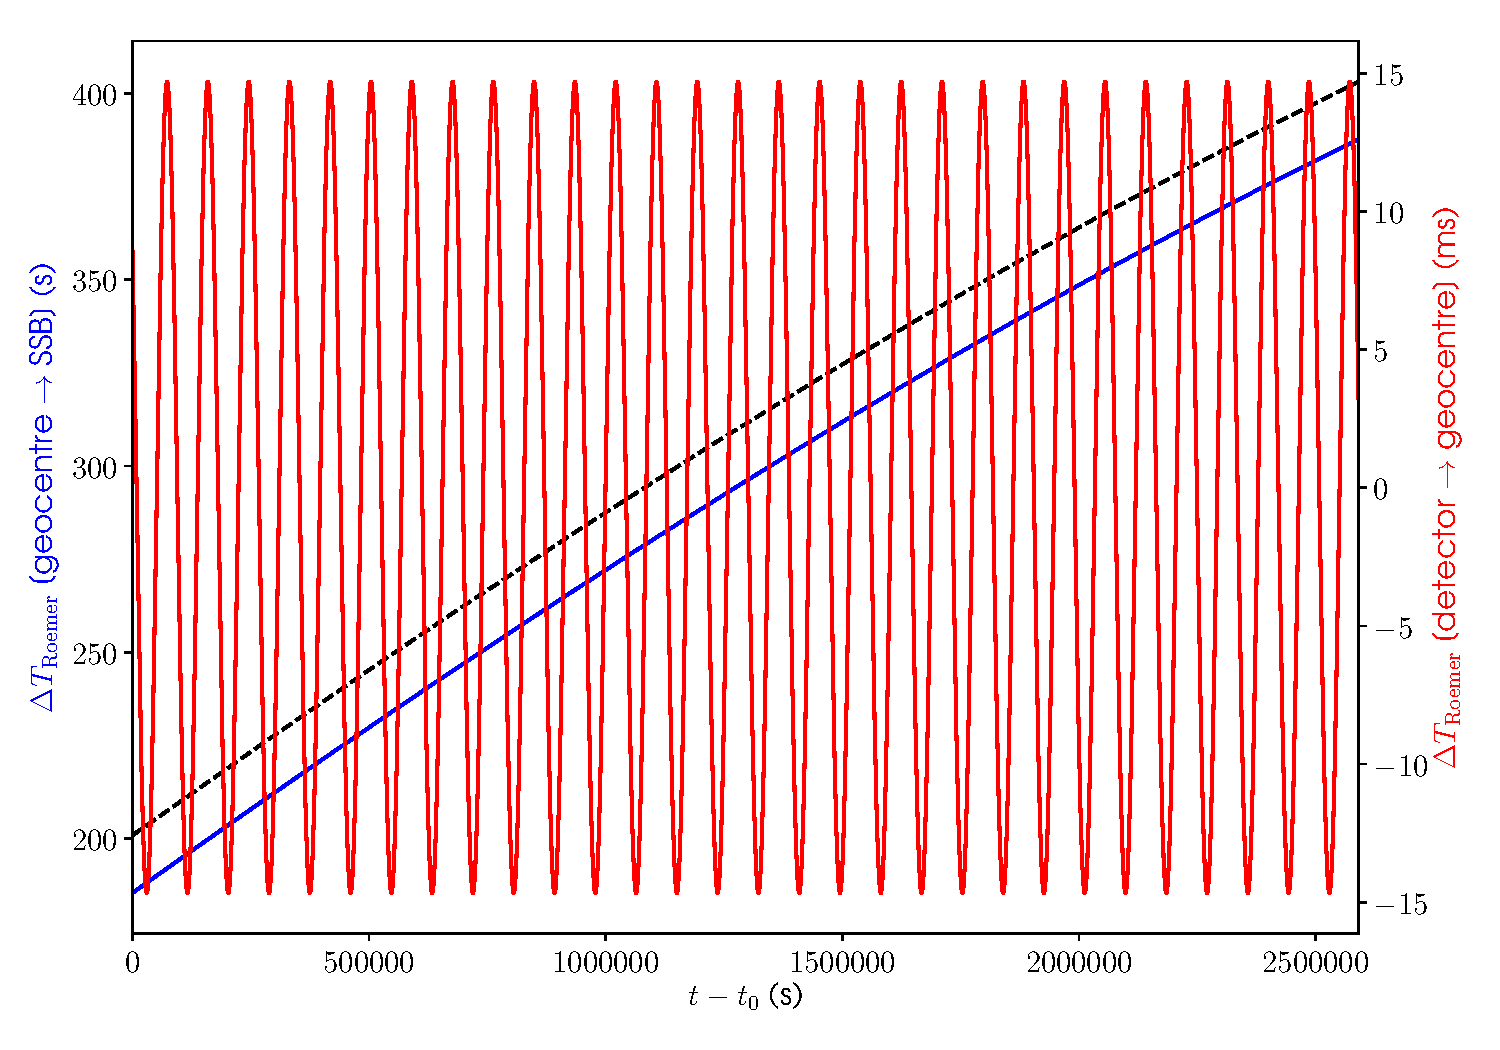
\includegraphics[keepaspectratio,width=\textwidth,height=170pt]{images/roemer_delay.pdf}
\label{roemer}
\end{figure}

\end{frame}

\begin{frame}

\frametitle{Background}
\label{background}

For long duration signals the phase needs to be tracked precisely -- time delay needs to be known
to $\mathcal{O}(\mu{\rm s})$ accuracy.

 %For an observation time of a year, and a signal at 100 Hz, sky locations
%separated by $15 \mu$ rad (near the ecliptic) produce 10% mismatches, so long wide-sky-area
%searches require the SSB calculation to be repeated for many sky positions. 

The code for the SSB calculation, e.g. \href{http://software.ligo.org/docs/lalsuite/lalpulsar/\_l\_a\_l\_barycenter\_8c\_source.html\#l00078}{\texttt{XLALBarycenterEarth()}}  and  \href{http://software.ligo.org/docs/lalsuite/lalpulsar/\_l\_a\_l\_barycenter\_8c\_source.html\#l00828}{\texttt{XLALBarycenter()}}, 
consists of many calls to \texttt{sin} and \texttt{cos}, so if needed many times this could be a computational bottleneck.

\textbf{Is there a way to speed up the calculation \emph{and} maintain accuracy?}

\end{frame}

\begin{frame}

\frametitle{Reduced Order Modelling}
\label{reducedordermodelling}

 \href{https://en.wikipedia.org/wiki/Model_order_reduction}{Reduced-order modelling}  (ROM) is basically a compression technique (similar to, e.g.,  \href{https://en.wikipedia.org/wiki/Principal_component_analysis}{Principal
Component Analysis} ).

\begin{itemize}
\item generate a ``training set'' of signal model vectors (each with length $M$) over a required parameter space

\item use modified  \href{https://en.wikipedia.org/wiki/Gram\%E2\%80\%93Schmidt\_process}{Gram-Schmidt process}  to form a
 minimal set of orthonormal bases from the ``training set'' that satisfy some constraint:

\begin{itemize}
\item a small projection error of the \emph{current} bases onto the remaining training data

\item a small \textbf{resdiual} when generating an interpolant from the current bases and
 comparing the interpolated models to the training set models

\end{itemize}

\end{itemize}

\end{frame}

\begin{frame}

\frametitle{Reduced Order Modelling}
\label{reducedordermodelling}

The set of $N$ \emph{reduced} orthonormal bases can then be used to form an interpolant:

\begin{itemize}
\item find $N$ best points (interpolation nodes) in the basis with which to form the interpolant

\item straightforward linear algebra to find a $N\times N$ matrix for interpolation

\end{itemize}

Linear algebra using the interpolant, the \emph{reduced} basis, and values of the full model function evaluated at only
the $N$ nodes (as opposed to $M$ points) gives an approximation of the full function at all $M$ points.

\end{frame}

\begin{frame}

\frametitle{Reduced Order Modelling}
\label{reducedordermodelling}

See, e.g., Appendix A \& B of \href{http://ukads.nottingham.ac.uk/abs/2013PhRvD..87l4005C}{Canizares \emph{et al}, PRD, 124005 (2013)}\footnote{\href{http://ukads.nottingham.ac.uk/abs/2013PhRvD..87l4005C}{http:/\slash ukads.nottingham.ac.uk\slash abs\slash 2013PhRvD..87l4005C}} for algorithms,
and \href{https://bitbucket.org/sfield83/greedycpp}{\texttt{greedycpp}}\footnote{\href{https://bitbucket.org/sfield83/greedycpp}{https:/\slash bitbucket.org\slash sfield83\slash greedycpp}} code for more details.

\end{frame}

\begin{frame}

\frametitle{Example analysis}
\label{exampleanalysis}

Form a reduced bases, and interpolant for any sky position, for the SSB time delay $\tau$ spanning
1 year for H1

\begin{itemize}
\item generate 2000 random sky positions $[\alpha, \delta]$ drawn uniformly over the sky

\item for each sky point calculate\footnote{excluding Shapiro delay due to cuspy nature} $\tau(t)$ over one year in 60 s steps (a $2000 \times 525960$ array)
 using \texttt{XLALBarycenterEarth()} and \texttt{XLALBarycenter()}

\item form a reduced basis with the constraint that the interpolant produces residual
 time delays of $< 0.1\mu{\rm s}$

\item validation and enrichment performed to fill in any sky gaps ($36\,000$ sky points tested
 in total)

\end{itemize}

\end{frame}

\begin{frame}

\frametitle{Example analysis}
\label{exampleanalysis}

Time delay (without Shapiro delay) can be reduced to 5 bases

\begin{figure}[htbp]
\centering
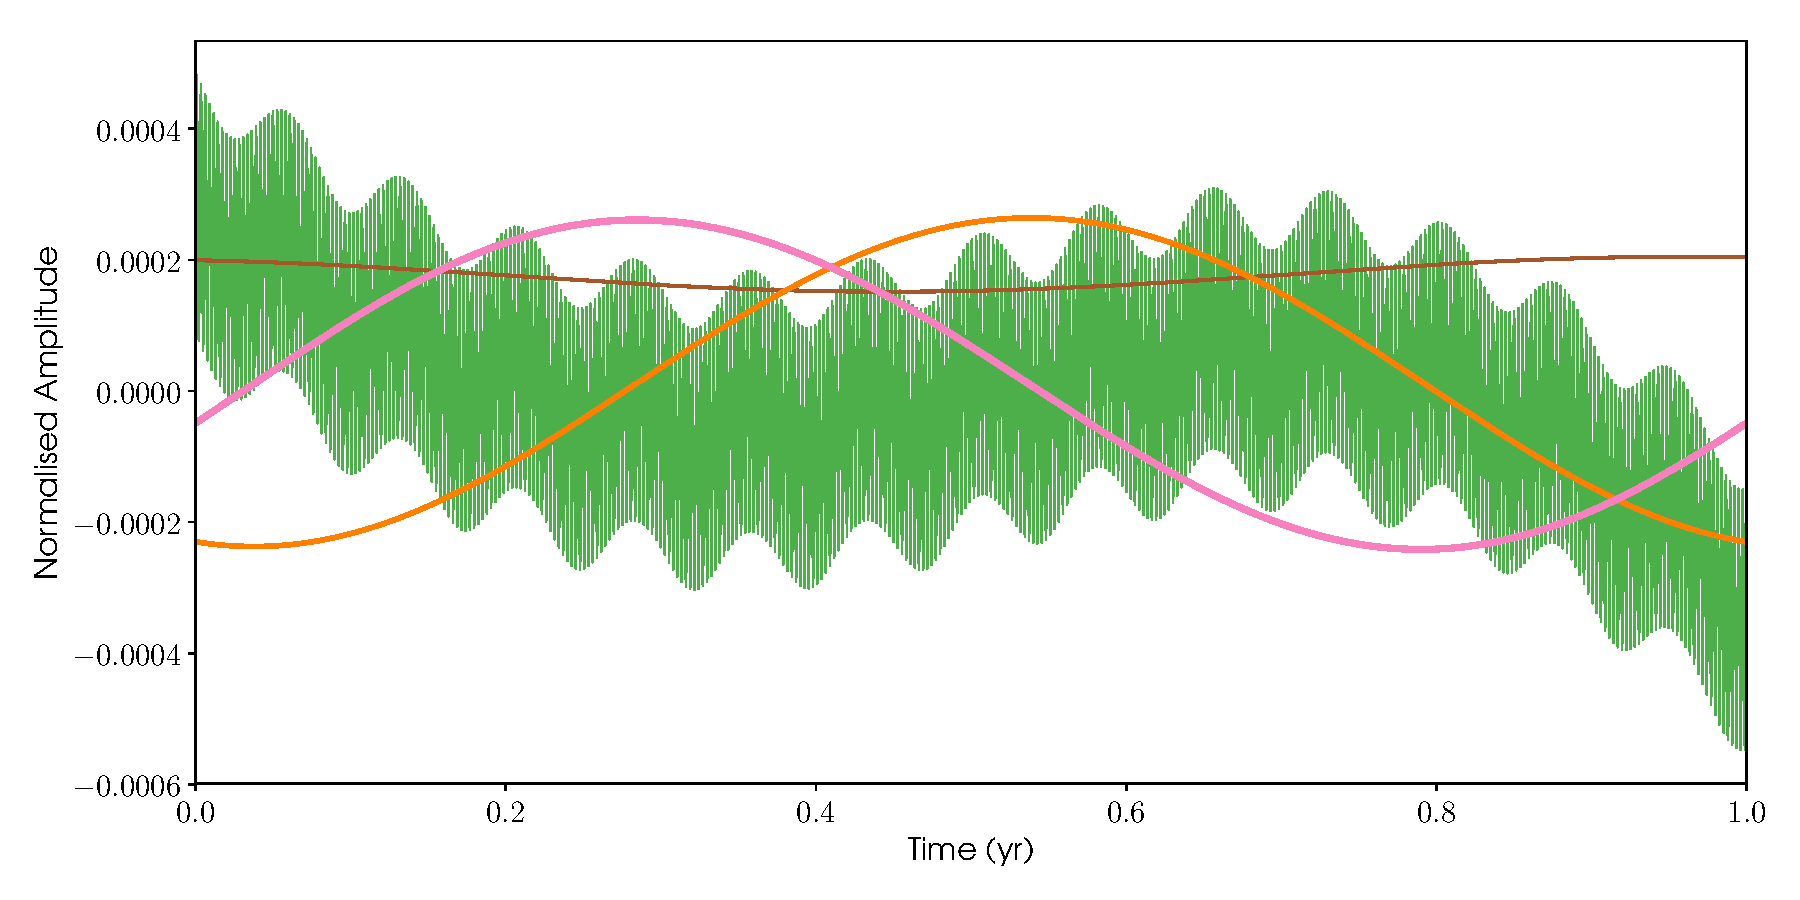
\includegraphics[keepaspectratio,width=\textwidth,height=200pt]{images/reduced_bases.pdf}
\label{bases}
\end{figure}

\end{frame}

\begin{frame}

\frametitle{Example analysis}
\label{exampleanalysis}

From the (now $525960 \times 5$) reduced basis, $\mathbf{B}$, calculate a $5\times 5$ interpolation matrix.

Then, for \textbf{any point in the sky}, we can produce an approximation of the time delay over a year by calculating
the delay using \texttt{XLALBarycenterEarth()} and \texttt{XLALBarycenter()} at only the 5 interpolation nodes.

See additional slides for linear algebra.

\end{frame}

\begin{frame}

\frametitle{Example analysis}
\label{exampleanalysis}

Therefore, we have 5 calls to the barycentring routines\footnote{\texttt{XLALBarycenterEarth()}+\texttt{XLALBarycenter()}} (plus some linear algebra) versus 525960 calls.

Using SWIG wrapped versions of the functions a single evaluation of the barycentring routines
takes\footnote{After initialising everything required. Setting the SWIG-wrapped \texttt{LIGOTimeGPS} structure
actually takes roughly as long as each call to the barycentering routines!} $\sim 1.2\!\times\!10^{-3}$ ms, whilst using \texttt{numpy} to perform the required linear algebra
for interpolation takes $\sim 3.1$ ms.

\begin{itemize}
\item Full calculation: $525960 \times 1.2\!\times\!10^{-3} \approx 630$ ms

\item ROM calculation: $(5 \times 1.2\!\times\!10^{-3}) + 3.1 \approx 3.1$ ms

\end{itemize}

There's roughly a 200 times speed-up!

\end{frame}

\begin{frame}

\frametitle{Example analysis}
\label{exampleanalysis}

\textbf{It can be quick, but is it accurate?}

\begin{figure}[htbp]
\centering
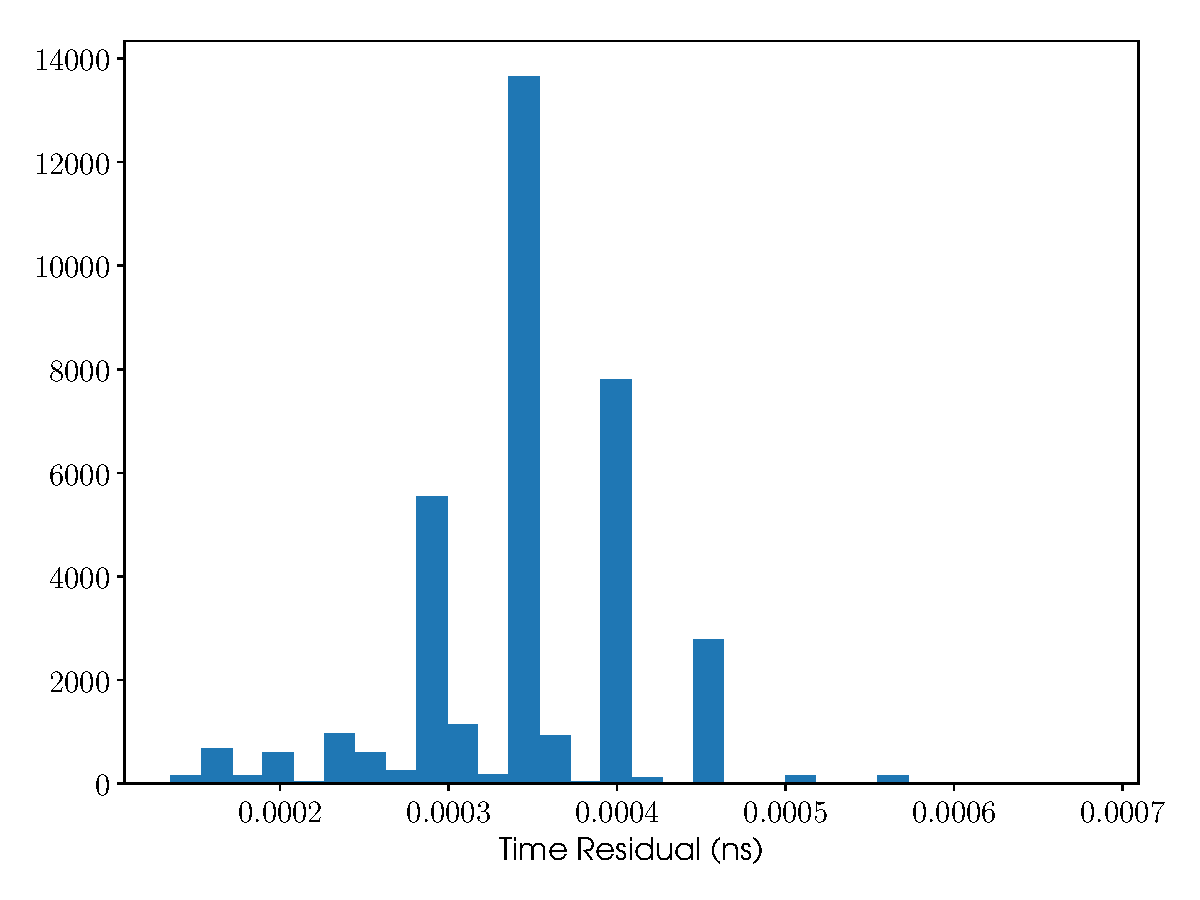
\includegraphics[keepaspectratio,width=\textwidth,height=190pt]{images/validation.pdf}
\label{validation}
\end{figure}

\end{frame}

\begin{frame}

\frametitle{Example analysis}
\label{exampleanalysis}

\textbf{But, what about Shapiro delay?}

Shapiro delay depends on sky position and detector location, but two main components of its calculation are sky
position independent, so can be computed once at an initialisation stage. 

For new sky positions these components then be used to calculate the full Shapiro delay over all times steps in the basis,
which (in \texttt{python})\footnote{This could probably be reduced if coded in \texttt{C}} takes $\sim 27$ ms.

So, when including Shapiro delay the ROM takes $\sim 30$ ms, which is an overall speed improvement of $\sim 20$.

\end{frame}

\begin{frame}

\frametitle{Example analysis}
\label{exampleanalysis}

Example residuals for a random sky location (including Shapiro delay)

\begin{figure}[htbp]
\centering
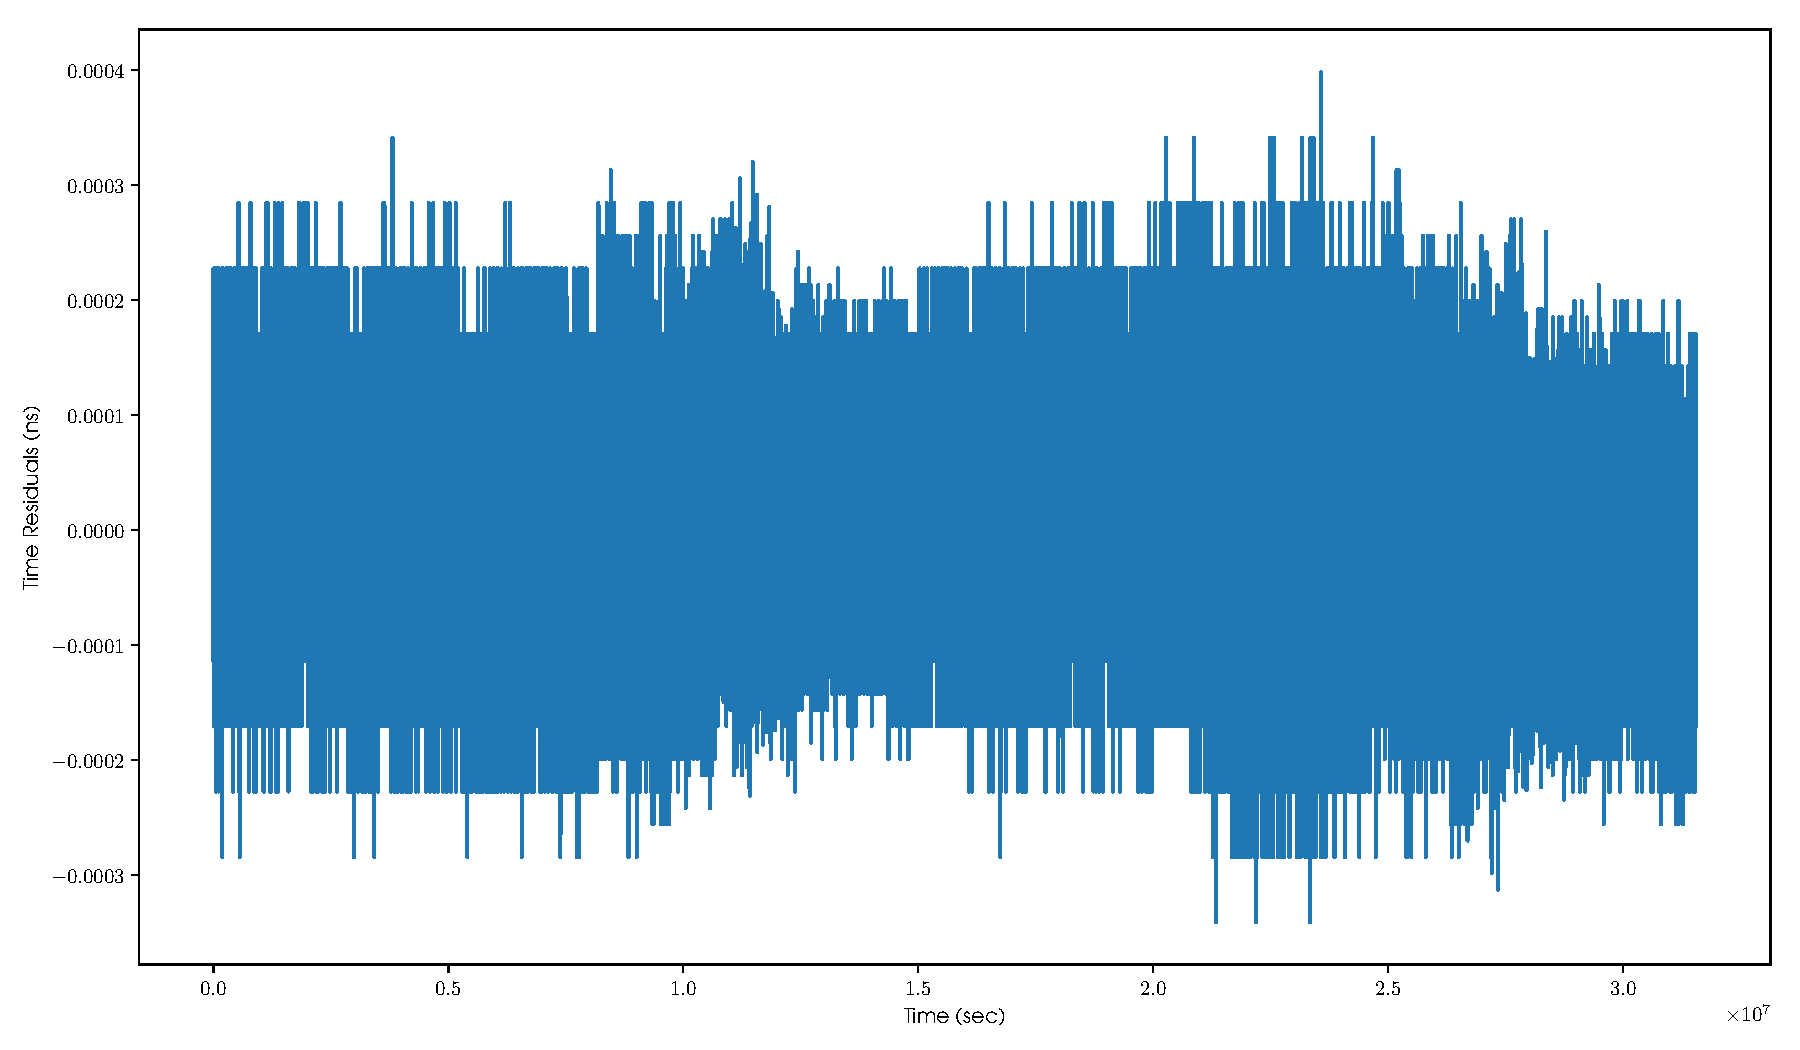
\includegraphics[keepaspectratio,width=\textwidth,height=170pt]{images/residuals.pdf}
\label{residuals}
\end{figure}

\end{frame}

\begin{frame}

\frametitle{Next steps}
\label{nextsteps}

\begin{itemize}
\item 5 basis vectors seem to be all that is required for day $\rightarrow$ month $\rightarrow$ year time-scales

\item create \texttt{LAL} functionality to use ROM for SSB calculation

\begin{itemize}
\item calculate reduced basis and interpolant matrices and nodes for successive year long time stretches

\item store matrices, nodes and sky locations of training models that produced the reduced basis

\item create initialisation function to reproduce the required reduced basis, and Shapiro delay
 components

\item create function to return a vector of times delays at a set of given GPS times (may use linear
 interpolation between basis set time steps)

\end{itemize}

\end{itemize}

\end{frame}

\begin{frame}

\frametitle{Usage}
\label{usage}

Although potentially not relevant for current all-sky searches, this could be useful for:

\begin{itemize}
\item \textbf{long coherent follow-ups} of candidates with broad sky error regions

\item searches that \textbf{stochasticly sample the sky} (e.g. using an MCMC) at many points

\end{itemize}

Reduced order modelling (and the related \emph{Reduced Order Quadrature} for likelihood calculations)
is already implemented (but, yet to be written-up!) in the standard Bayesian pipeline known pulsar search
for narrow parameter searches including frequency and binary parameters.

\end{frame}

\begin{frame}

\frametitle{Future}
\label{future}

Even if this has limited applicability in current CW searches it may be relevant in other cases:

\begin{itemize}
\item CBC signals may need days-long templates in 3G detector era that require referencing to SSB

\item Many signals in LISA require referencing to the SSB

\item PTAs currently have quite sparse time samples, but in the future (e.g. SKA) there may be larger
 numbers of samples

\end{itemize}

\end{frame}

\begin{frame}

\frametitle{Acknowlegdments}
\label{acknowlegdments}

Rory Smith has provided invaluable information on Reduced Order Modelling.

Initial stages of this work were performed by two undergraduate students: Stuart Doolan
and Lisa McMenanmin.

I am grateful to Scott Field and the other developers of \href{https://bitbucket.org/sfield83/greedycpp}{\texttt{greedycpp}}\footnote{\href{https://bitbucket.org/sfield83/greedycpp}{https:/\slash bitbucket.org\slash sfield83\slash greedycpp}}.

The modified version of \texttt{greedycpp} used for this analysis can be found \href{https://github.com/mattpitkin/greedycpp/tree/redordbar/}{here}\footnote{\href{https://github.com/mattpitkin/greedycpp/tree/redordbar/}{https:/\slash github.com\slash mattpitkin\slash greedycpp\slash tree\slash redordbar\slash }}.

\end{frame}

\begin{frame}

\frametitle{Additional slides: linear algebra}
\label{additionalslides:linearalgebra}

We have an $M \times N$ reduced basis matrix $\mathbf{B}$, where $M$ is the length of each base and $N$ is the number of bases.
Due to their orthonomality we know that a linear combination of bases should be able to produce an approximation to any \emph{true}
full model. If we have $N$ nodes that are optimal points for interpolation, then we can calculate the coefficients $\vec{C}$ of the
linear superposition of bases:
 \begin{align}
\vec{t} &= \vec{C}~\mathbf{b}, \nonumber \\
\vec{C} &= \vec{t}~\mathbf{b}^{-1} \nonumber
\end{align} 
where $\vec{t}$ is the vector of model values computed at the $N$ nodes, and $\mathbf{b}$ is an $N \times N$ matrix of the reduced
basis values at the $N$ nodes.

\end{frame}

\begin{frame}

\frametitle{Additional slides: linear algebra}
\label{additionalslides:linearalgebra}

We can then form the full model vector (at all $M$ points) with
\[
\vec{T} = \vec{C}~\mathbf{B}.
\]

Alternatively, we can reorder this, given that $\vec{C} = \vec{t}~\mathbf{b}^{-1}$, so that
\[
\vec{T} = \vec{t}\,(\mathbf{b}^{-1}~\mathbf{B}),
\]
where the $\mathbf{b}^{-1}~\mathbf{B}$ part can be precomputed.

\end{frame}

\mode<all>
\input{mmd-beamer-footer}

\end{document}\mode*

